\subsection{Data-Efficient Noise Modeling}
\label{sec:jiModeling}

A procedure for optimizing manufacturer-provided noise models to active quantum computing systems is provided in Ji et al.
This model learns parameters associated with stochastic, coherent, non-Markovian, and correlated sources for both one- and two-qubit operations. %, shown in Table \ref{tab:jiparameters}.
Rather than starting from guessed or random noise parameters, the suggested framework starts from a reference characterization such as a vendor-calibrated baseline model.
Due to the computational inefficiency of brute force search for optimal parameter fitting, Bayesian Optimization using a tree-structured Parzen estimator is used to tune the noise parameters.
The cost function for training is the Hellinger distance between measured and simulated output distributions.
% \begin{equation}
%     \theta^* = \text{argmin}_{\theta} \left( \frac{1}{|C|} \sum_{i} H[P_i, Q_i(\theta)] \right)
%     \label{eq:optimal_theta}
% \end{equation}

Using already existing parameters to speed up characterization reduces the time and hardware resources required to train the noise model.
The use of reference parameters also ``allows for the continuous refinement of noise models, ensuring scalability for larger quantum circuits and processors'' \cite{ji_data-efficient_2025}.

% \begin{quote}
%     A key advantage of our approach is its efficiency and practicality.
%     It repurposes existing benchmarking or application-specific execution data, avoiding the need for extensive characterization protocols such as quantum  process tomography.
%     This reusability reduces experimental overhead, enabling practitioners to leverage prior executions to improve algorithm testing and error mitigation protocols.
%     Moreover, this allows for the continuous refinement of noise models, ensuring scalability for larger quantum circuits and processors.
%     \cite{ji_data-efficient_2025}.
% \end{quote}


% \begin{table}[b]
    \centering
    \begin{tabular}{llc}
        \hline
        \textbf{Parameter} & \textbf{Description} & \textbf{Type} \\
        \hline
        \multicolumn{3}{c}{\textbf{Single-Qubit Gate Parameters (7)}} \\
        $k_{\text{dep}}$ & Depolarizing scaling factor & Stochastic \\
        $b_{\text{dep}}$ & Depolarizing offset & Stochastic \\
        $b_{\text{amp}}$ & Amplitude damping offset & Stochastic \\
        $\theta_{x,y,z}$ & Coherent rotation angles & Coherent \\
        $\beta_{1\text{Q}}$ & Stretched dephasing exponent & Non-Markovian \\
        \hline
        \multicolumn{3}{c}{\textbf{Two-Qubit Gate Parameters (9)}} \\
        $k_{\text{dep,2Q}}$ & Depolarizing scaling factor & Stochastic \\
        $b_{\text{dep,2Q}}$ & Depolarizing offset & Stochastic \\
        $b_{\text{amp,2Q}}$ & Amplitude damping offset & Stochastic \\
        $b_{\phi,2Q}$ & Phase damping offset & Stochastic \\
        $\theta_{\text{ixx,yy,zz}}$ & Coherent crosstalk angles & Coherent \\
        $\beta_{2\text{Q}}$ & Stretched dephasing exponent & Non-Markovian \\
        $k_{zz}$ & Correlated ZZ dephasing rate & Correlated \\
        \hline
        \multicolumn{3}{c}{\textbf{Correlated Readout Parameters (4)}} \\
        $a, b_{00\leftrightarrow 11}$ & Coefficients (\textbar 00 \textgreater \(\leftrightarrow\) \textbar 11 \textgreater) & Correlated \\
        $a, b_{01\leftrightarrow 10}$ & Coefficients (\textbar 01 \textgreater \(\leftrightarrow\) \textbar 10 \textgreater) & Correlated \\
        \hline
    \end{tabular}
    \caption{Gate and readout parameters as described in \cite{ji_data-efficient_2025}}
    \label{tab:jiparameters}
\end{table}

\begin{figure}
    \centering
    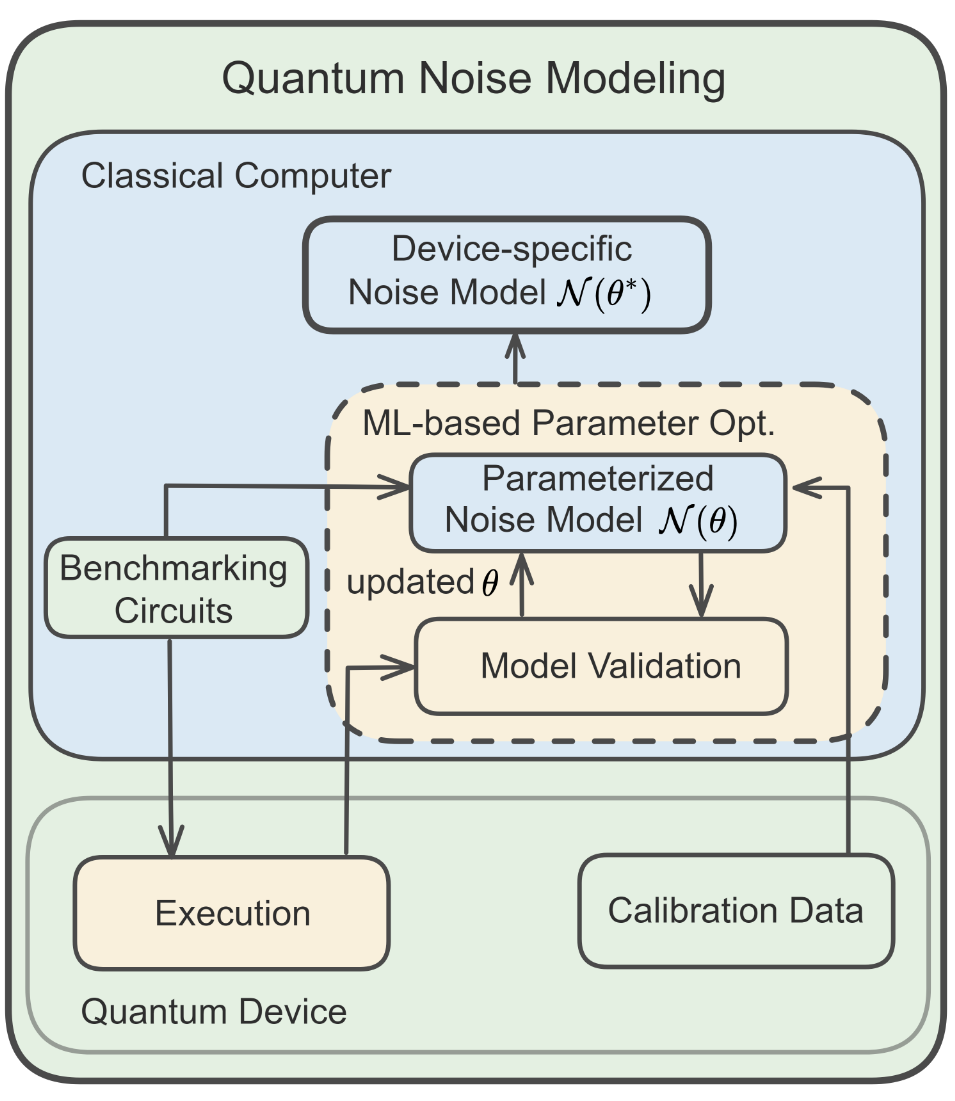
\includegraphics[width=0.5\linewidth]{figures/jie_framework.png}
    \caption{Framework outline for noise modeling in section \ref{sec:jiModeling}}
    \label{fig:ji_framework}
\end{figure}

